\documentclass[11pt,a4paper]{ctexart}
\usepackage{common/ipara}

\definecolor{gold}{RGB}{218,165,32}
\tikzset{
  geom/.style={thick,draw=blue!80!black},
  aid/.style={thin,draw=gray!60},
  hline/.style={thick,draw=gold!90!black},
  vline/.style={thick,draw=teal,->,>=stealth},
  vpoint/.style={circle,fill=black,inner sep=1.2pt},
  centerpt/.style={circle,fill=gray!80,inner sep=1.2pt},
  moving/.style={circle,fill=gold!90!black,inner sep=1.5pt}
}

\newcommand{\vect}[1]{\overrightarrow{#1}}

\newcommand{\figcap}[2]{%
  \begin{center}\begin{minipage}{.92\linewidth}\centering
  \ifx&#1&\else#1\fi
  \ifx&#2&\else\ifx&#1&\else\\[-.35em]\fi{\footnotesize\color{gray}#2}\fi
  \end{minipage}\end{center}}

% --- Figure 1: Cartesian Coordinates with Origin at Circle Center O(0,0) ---
\newcommand{\figEquilateralCoord}{%
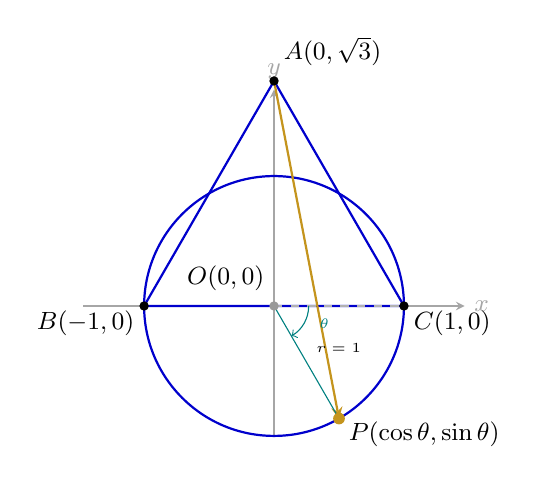
\begin{tikzpicture}[scale=1.1,every node/.style={font=\small}]
  \draw[->,>=stealth,gray!70] (-2.2,0)--(2.2,0) node[right] {$x$};
  \draw[->,>=stealth,gray!70] (0,-1.5)--(0,2.5) node[above] {$y$};
  \coordinate (O) at (0,0); \coordinate (B) at (-1.5,0); \coordinate (C) at (1.5,0);
  \coordinate (A) at (0,2.598); \coordinate (P) at (0.75,-1.299);
  \draw[geom] (O) circle (1.5);
  \draw[geom] (A)--(B)--(C)--cycle;
  \draw[vline,draw=gold!90!black] (A)--(P);
  \draw[aid,draw=teal] (O)--(P) node[midway,above right,font=\tiny] {$r=1$};
  \draw[aid,dashed] (O)--(1.5,0);
  \draw[teal,->] (0.4,0) arc[start angle=0, end angle=-60, radius=0.4] node[midway,right=2pt,font=\tiny] {$\theta$};
  \node[centerpt,label={[above left]$O(0,0)$}] at (O){};
  \node[vpoint,label={[above right]$A(0,\sqrt{3})$}] at (A){};
  \node[vpoint,label={[below left]$B(-1,0)$}] at (B){};
  \node[vpoint,label={[below right]$C(1,0)$}] at (C){};
  \node[moving,label={[below right]$P(\cos\theta,\sin\theta)$}] at (P){};
\end{tikzpicture}}

% --- Figure 2: Vector Projection (For Method 2) ---
\newcommand{\figEquilateralProj}{%
\begin{tikzpicture}[scale=.78,every node/.style={font=\small}]
  \coordinate (B) at (-2,0); \coordinate (C) at (2,0); \coordinate (A) at (0,3.464); \coordinate (O) at (0,0);
  \coordinate (P) at (1,-1.732);
  \draw[geom] (O) circle (2);
  \draw[geom] (A)--(B)--(C)--cycle;
  \draw[vline,draw=gold!90!black] (A)--(P);
  \draw[aid,draw=teal,thick,->,>=stealth] (A)--(C) node[midway,above right,font=\scriptsize,text=teal] {向量 \(\vec c = \vect{AC}\)};
  \draw[aid,dashed,draw=teal] (O)--(P) node[midway,above left,font=\scriptsize] {\(\vect{OP} \parallel \vec c\)};
  \node[vpoint,label=above:$A$] at (A){}; \node[vpoint,label=left:$B$] at (B){}; \node[vpoint,label=right:$C$] at (C){};
  \node[moving,label=below right:$P$] at (P){}; \node[centerpt,label=above left:$O$] at (O){};
\end{tikzpicture}}

% --- Figure 3: Equal-Sum Line & Tangent Point (For Method 3) ---
\newcommand{\figEquilateralDiameter}{%
\begin{tikzpicture}[scale=.78,every node/.style={font=\small}]
  \coordinate (B) at (-2,0); \coordinate (C) at (2,0); \coordinate (A) at (0,3.464); \coordinate (O) at (0,0);
  \coordinate (C0) at (1,1.732); \coordinate (P) at (1,-1.732);
  \draw[geom] (O) circle (2);
  \draw[geom] (A)--(B)--(C)--cycle;
  \draw[aid] (-2.5,-0.288)--(1.6,2.078) node[right,font=\scriptsize,text=gray!70!black] {等和基线 \(\lambda+2\mu=1\)};
  \draw[hline] (-0.8,-2.771)--(2.8,-0.693) node[right,font=\scriptsize,text=gold!90!black] {等和切线 \(\lambda+2\mu=\frac{5}{2}\)};
  \draw[vline,draw=gold!90!black] (A)--(P);
  \draw[aid,draw=teal] (O)--(P);
  \node[vpoint,label=above:$A$] at (A){}; \node[vpoint,label=left:$B$] at (B){}; \node[vpoint,label=right:$C$] at (C){};
  \node[moving,label=below right:$P$] at (P){}; \node[centerpt,label=above left:$O$] at (O){};
  \node[vpoint,label=right:$C_0$] at (C0){};
\end{tikzpicture}}

\begin{document}

\begin{center}
  {\Large\bfseries\sffamily 作业解答}
\end{center}

\vspace{0.3em}
\subsection*{解法一：三角参数法（高考通用建系法——推荐）}
为了简化圆的方程，设等边三角形边长 \(a=2\)。取直径 \(BC\) 的中点（圆心）\(O(0,0)\) 为直角坐标系原点，以 \(BC\) 所在直线为 \(x\) 轴，高线 \(OA\) 所在直线为 \(y\) 轴建立平面直角坐标系。

由于 \(BC=2\)，故 \(B,C\) 坐标为 \(B(-1,0), C(1,0)\)。等边三角形的高 \(h = 2 \cdot \sin 60^\circ = \sqrt{3}\)，故顶点 \(A(0,\sqrt{3})\)。
圆 \(BC\) 的圆心为原点 \(O(0,0)\)，半径 \(r=1\)，其标准方程为 \(x^2+y^2=1\)。

设圆上任意动点 \(P(\cos\theta, \sin\theta)\)，其中旋转角 \(\theta \in [0, 2\pi)\)。

\figcap{\figEquilateralCoord}{解法一图解：建立以圆心 \(O(0,0)\) 为原点的直角坐标系与圆的参数表示}

根据向量坐标定义，各点相对于基点 \(A(0,\sqrt{3})\) 的位置向量为：
\[
\vect{AP} = P - A = (\cos\theta, \sin\theta-\sqrt{3}),\quad \vect{AB} = B - A = (-1,-\sqrt{3}),\quad \vect{AC} = C - A = (1,-\sqrt{3}).
\]
按题意展开向量线性组合方程 \(\vect{AP} = \lambda\vect{AB} + \mu\vect{AC}\)：
\[
(\cos\theta, \sin\theta-\sqrt{3}) = \lambda (-1,-\sqrt{3}) + \mu (1,-\sqrt{3}) = (-\lambda+\mu, -\sqrt{3}\lambda-\sqrt{3}\mu).
\]
对比 \(x,y\) 分量可得二元一次方程组：
\[
\begin{cases}
  -\lambda + \mu = \cos\theta, & \text{--- (式 \uppercase\expandafter{\romannumeral 1})}\\[0.3em]
  -\sqrt{3}\lambda - \sqrt{3}\mu = \sin\theta - \sqrt{3} \implies \lambda+\mu = 1 - \frac{\sin\theta}{\sqrt{3}}. & \text{--- (式 \uppercase\expandafter{\romannumeral 2})}
\end{cases}
\]
两式相加除以 \(2\) 得 \(\mu = \frac{1}{2}\cos\theta - \frac{1}{2\sqrt{3}}\sin\theta + \frac{1}{2}\)；
由 (式 \uppercase\expandafter{\romannumeral 2}) 减去 (式 \uppercase\expandafter{\romannumeral 1}) 除以 \(2\) 得 \(\lambda = -\frac{1}{2}\cos\theta - \frac{1}{2\sqrt{3}}\sin\theta + \frac{1}{2}\)。

将 \(\lambda,\mu\) 代入目标表达式 \(\lambda+2\mu\) 并利用辅助角公式化简：
\[
\begin{aligned}
\lambda+2\mu &= \left(-\frac{1}{2}\cos\theta - \frac{1}{2\sqrt{3}}\sin\theta + \frac{1}{2}\right) + 2\left(\frac{1}{2}\cos\theta - \frac{1}{2\sqrt{3}}\sin\theta + \frac{1}{2}\right)\\[0.5em]
&= \frac{1}{2}\cos\theta - \frac{\sqrt{3}}{2}\sin\theta + \frac{3}{2}\\[0.5em]
&= \cos\left(\theta + 60^\circ\right) + \frac{3}{2}.
\end{aligned}
\]
因为 \(\theta \in [0, 2\pi)\)，所以相角 \(\theta+60^\circ \in [60^\circ, 420^\circ]\)，完整覆盖三角函数的单值单周期。
当 \(\theta+60^\circ = 360^\circ\)（即 \(\theta = 300^\circ\)）时，\(\cos(\theta+60^\circ) = 1\) 取得最大值：
\[
\max(\lambda+2\mu) = 1 + \frac{3}{2} = \mathbf{\frac{5}{2}}.
\]

\vspace{1em}
\subsection*{解法二：向量投影法（几何最简法）}
设等边三角形边长为 \(a\)，记基底向量 \(\vec b = \vect{AB}, \vec c = \vect{AC}\)。因为 \(\triangle ABC\) 为等边三角形，
\[
|\vec b|=|\vec c|=a,\qquad \vec b\cdot\vec c = a \cdot a \cdot \cos 60^\circ = \frac{a^2}{2}.
\]
由条件 \(\vect{AP} = \lambda\vec b + \mu\vec c\)，两边同时与 \(\vec c\) 做点乘（数量积）：
\[
\vect{AP}\cdot\vec c = \lambda (\vec b\cdot\vec c) + \mu (\vec c\cdot\vec c) = \lambda \frac{a^2}{2} + \mu a^2 = \frac{a^2}{2}(\lambda+2\mu).
\]
变形分离目标加权和，得到\textbf{数量积与加权和的等价转换公式}：
\[
\lambda+2\mu = \frac{2}{a^2} \left(\vect{AP}\cdot\vec c\right).
\]
求 \(\lambda+2\mu\) 的最大值等价于求向量 \(\vect{AP}\) 在 \(\vec c\) 方向上的数量积（即投影）最大值。

\figcap{\figEquilateralProj}{解法二图解：将加权和转化为 \(\vect{AP}\) 在 \(\vec c\) 方向上的向量投影}

设 \(O\) 为 \(BC\) 中点（圆心），由中点公式有 \(\vect{AO} = \frac{\vec b+\vec c}{2}\)，圆半径 \(r = |\vect{OP}| = \frac{a}{2}\)。
拆分向量 \(\vect{AP} = \vect{AO} + \vect{OP}\) 代入数量积：
\[
\vect{AP}\cdot\vec c = (\vect{AO} + \vect{OP})\cdot\vec c = \vect{AO}\cdot\vec c + \vect{OP}\cdot\vec c.
\]
计算固定项 \(\vect{AO}\cdot\vec c\)：
\[
\vect{AO}\cdot\vec c = \frac{\vec b+\vec c}{2}\cdot\vec c = \frac{\vec b\cdot\vec c + |\vec c|^2}{2} = \frac{\frac{a^2}{2} + a^2}{2} = \frac{3a^2}{4}.
\]
对于动项 \(\vect{OP}\cdot\vec c\)，当 \(\vect{OP}\) 与 \(\vec c\) 方向完全一致（即 \(\vect{OP} \parallel \vec c\) 且同向）时取最大值：
\[
\max(\vect{OP}\cdot\vec c) = |\vect{OP}| \cdot |\vec c| = \frac{a}{2} \cdot a = \frac{a^2}{2}.
\]
故 \(\max(\vect{AP}\cdot\vec c) = \frac{3a^2}{4} + \frac{a^2}{2} = \frac{5a^2}{4}\)。代回转换公式：
\[
\max(\lambda+2\mu) = \frac{2}{a^2} \cdot \frac{5a^2}{4} = \mathbf{\frac{5}{2}}.
\]

\vspace{1em}
\subsection*{解法三：等和线法（几何直观法）}
设边长 \(a=2\)，记 \(\vec b = \vect{AB}, \vec c = \vect{AC}\)。

1. \textbf{确定等和基线 \(L_1\) 的几何位置}：
   等和基线方程 \(L_1: \lambda+2\mu=1\)。
   当 \(\mu=0\) 时 \(\lambda=1 \implies B(1,0)\) 点在基线上；
   当 \(\lambda=0\) 时 \(\mu=1/2 \implies AC\) 的中点 \(C_0(0,1/2)\) 点在基线上。
   故基线 \(L_1\) 为连接 \(B\) 与 \(AC\) 中点 \(C_0\) 的直线 \(BC_0\)。

2. \textbf{证明基线与 \(AC\) 垂直}：
   在 \(\triangle AB C_0\) 中，\(AB=2\)，\(C_0\) 为 \(AC\) 中点故 \(AC_0 = 1\)，且夹角 \(\angle A = 60^\circ\)。
   由余弦定理计算 \(BC_0\) 长度：
   \[
   BC_0^2 = AB^2 + AC_0^2 - 2 AB \cdot AC_0 \cos 60^\circ = 2^2 + 1^2 - 2(2)(1)\left(\frac{1}{2}\right) = 3.
   \]
   注意到 \(BC_0^2 + AC_0^2 = 3 + 1 = 4 = AB^2\)，由勾股定理逆定理可知 \(\angle AC_0B = 90^\circ\)，即\textbf{基线 \(BC_0 \perp AC\)}。

3. \textbf{平移切线求最大值}：
   等和线簇 \(L_k: \lambda+2\mu=k\) 均为平行于 \(BC_0\) 的直线，即都垂直于 \(AC\)。

\figcap{\figEquilateralDiameter}{解法三图解：等和切线 \(L_k\) 平移相切于点 \(P\)}

当等和线 \(L_k\) 向右下方平移至与圆相切于点 \(P\) 时，\(k\) 取得最大值。此时切点半径 \(\vect{OP}\) 必垂直于切线 \(L_k\)，故 \(\vect{OP} \parallel \vect{AC}\)。
圆心 \(\vect{AO} = \frac{1}{2}\vec b + \frac{1}{2}\vec c\)，半径向量 \(\vect{OP} = \frac{1}{2}\vect{AC} = \frac{1}{2}\vec c\)。
切点向量为：
\[
\vect{AP} = \vect{AO} + \vect{OP} = \left(\frac{1}{2}\vec b + \frac{1}{2}\vec c\right) + \frac{1}{2}\vec c = \frac{1}{2}\vec b + 1\vec c \implies \lambda = \frac{1}{2},\ \mu = 1.
\]
代入目标式得：\(\max(\lambda+2\mu) = \frac{1}{2} + 2(1) = \mathbf{\frac{5}{2}}\)。

\vspace{1em}
\subsection*{解法四：直角坐标系与圆上线性函数公式法}
同解法一，建立以圆心 \(O(0,0)\) 为原点的坐标系，圆方程为 \(x^2+y^2=1\)。
动点 \(P(x,y)\) 满足 \(\vect{AP} = (x, y-\sqrt{3})\)。
由 \(\vect{AP} = \lambda(-1,-\sqrt{3}) + \mu(1,-\sqrt{3})\) 解出的坐标转换关系：
\[
\begin{cases}
  x = -\lambda + \mu\\[0.3em]
  y - \sqrt{3} = -\sqrt{3}(\lambda+\mu) \implies \lambda+\mu = 1 - \frac{y}{\sqrt{3}}
\end{cases}
\implies
\begin{cases}
  \mu = \frac{1}{2}x - \frac{y}{2\sqrt{3}} + \frac{1}{2}\\[0.3em]
  \lambda = -\frac{1}{2}x - \frac{y}{2\sqrt{3}} + \frac{1}{2}
\end{cases}
\]
代入目标式导出直角坐标下的线性函数：
\[
\lambda+2\mu = \frac{1}{2}x - \frac{\sqrt{3}}{2}y + \frac{3}{2}.
\]
问题转化为求 \(f(x,y) = \frac{1}{2}x - \frac{\sqrt{3}}{2}y + \frac{3}{2}\) 在单位圆 \(x^2+y^2=1\) 上的最大值。

应用圆上线性函数最大值通式 \(\max(ax+by) = r\sqrt{a^2+b^2}\)（其中 \(a=\frac{1}{2}, b=-\frac{\sqrt{3}}{2}, r=1\)）：
\[
\max\left(\frac{1}{2}x - \frac{\sqrt{3}}{2}y\right) = 1 \cdot \sqrt{\left(\frac{1}{2}\right)^2 + \left(-\frac{\sqrt{3}}{2}\right)^2} = \sqrt{\frac{1}{4} + \frac{3}{4}} = 1.
\]
故 \(\max(\lambda+2\mu) = 1 + \frac{3}{2} = \mathbf{\frac{5}{2}}\)。

\vspace{1em}
\subsection*{解法五：二次方程判别式法（切线判别式）}
以圆心 \(O(0,0)\) 为原点，圆方程为 \(x^2+y^2=1\)。
由解法四导出的线性关系 \(\lambda+2\mu = \frac{1}{2}x - \frac{\sqrt{3}}{2}y + \frac{3}{2}\)，设目标值为 \(t = \lambda+2\mu\)。
同乘以 \(2\) 移项解出 \(x\)：
\[
2t - 3 = x - \sqrt{3}y \implies x = \sqrt{3}y + (2t - 3).
\]
将 \(x\) 代入圆方程 \(x^2+y^2=1\) 中，消去 \(x\) 得到关于 \(y\) 的一元二次方程：
\[
\left[\sqrt{3}y + (2t - 3)\right]^2 + y^2 = 1 \iff 4y^2 + 2\sqrt{3}(2t - 3)y + (2t - 3)^2 - 1 = 0.
\]
因为动点 \(P(x,y)\) 在圆上，直线 \(x - \sqrt{3}y + \frac{3}{2} - t = 0\) 与圆必有公共点，故二次方程在 \(y \in [-1,1]\) 内必有实根，判别式 \(\Delta \ge 0\)：
\[
\Delta = \left[2\sqrt{3}(2t - 3)\right]^2 - 4 \cdot 4 \cdot \left[(2t - 3)^2 - 1\right] \ge 0.
\]
化简得：
\[
12(2t - 3)^2 - 16(2t - 3)^2 + 16 \ge 0 \iff -4(2t - 3)^2 + 16 \ge 0 \iff (2t - 3)^2 \le 4.
\]
开方解不等式：
\[
-2 \le 2t - 3 \le 2 \implies 1 \le 2t \le 5 \implies \frac{1}{2} \le t \le \mathbf{\frac{5}{2}}.
\]

\vspace{1em}
\subsection*{解法六：直径圆条件与二次型配方法}
记 \(\vec b = \vect{AB}, \vec c = \vect{AC}\)。因为 \(P\) 在以 \(BC\) 为直径的圆上，由圆的几何性质，\(\angle BPC = 90^\circ \iff \vect{PB}\perp\vect{PC} \iff \vect{PB}\cdot\vect{PC} = 0\)。
用基底 \(\vec b, \vec c\) 表示向量 \(\vect{PB}\) 与 \(\vect{PC}\)：
\[
\vect{PB} = \vect{AB} - \vect{AP} = \vec b - (\lambda\vec b + \mu\vec c) = (1-\lambda)\vec b - \mu\vec c,
\]
\[
\vect{PC} = \vect{AC} - \vect{AP} = \vec c - (\lambda\vec b + \mu\vec c) = -\lambda\vec b + (1-\mu)\vec c.
\]
将两向量代入数量积 \(\vect{PB}\cdot\vect{PC} = 0\) 展开：
\[
[(1-\lambda)\vec b - \mu\vec c] \cdot [-\lambda\vec b + (1-\mu)\vec c] = 0.
\]
利用 \(|\vec b|^2=a^2, |\vec c|^2=a^2, \vec b\cdot\vec c = \frac{a^2}{2}\) 展开并两边同除以 \(a^2\)：
\[
-\lambda(1-\lambda) + (1-\lambda)(1-\mu)\frac{1}{2} + \lambda\mu\frac{1}{2} - \mu(1-\mu) = 0.
\]
同乘以 \(2\) 化简整理，得到 \(\lambda,\mu\) 满足的二次型约束方程：
\[
2\lambda^2 + 2\lambda\mu + 2\mu^2 - 3\lambda - 3\mu + 1 = 0.
\]
令 \(u = \lambda-\frac{1}{2}, v = \mu-\frac{1}{2}\) 进行中心平移，约束方程简化为标准二次型：\(u^2 + uv + v^2 = \frac{1}{4}\)。
目标代数式为 \(\lambda+2\mu = \left(u+\frac{1}{2}\right) + 2\left(v+\frac{1}{2}\right) = \frac{3}{2} + (u+2v)\)。
利用代数恒等式配方：
\[
4(u^2+uv+v^2) - (u+2v)^2 = 3u^2 \ge 0 \implies (u+2v)^2 \le 4(u^2+uv+v^2) = 1.
\]
解得 \(u+2v \le 1\)，故 \(\max(\lambda+2\mu) = \frac{3}{2} + 1 = \mathbf{\frac{5}{2}}\)。

\end{document}
